\documentclass[10pt,a4paper, twocolumn]{article}
\usepackage[utf8]{inputenc}
\usepackage[english]{babel}
\usepackage{amsmath}
\usepackage{amsfonts}
\usepackage{amssymb}
\usepackage{lmodern}
\usepackage{amsthm}
\usepackage{graphicx}

\usepackage[left=2cm,right=2cm,top=2cm,bottom=2cm]{geometry}
\author{Mehdi Bahri}
\title{Dynamical Systems and Deep Learning - Coursework II}

\theoremstyle{definition}
\newtheorem{defn}{Definition}

\begin{document}
\maketitle
\section{Methodology}
In this experiment, we try different ways of finding suitable hyperparameters for a neural network made from a single RBM. We measure the performance of the RBM on the \texttt{Caltech 101 figures} dataset. The quality metric we are trying to optimise is the prediction error of the RBM on a fixed testing set.

\vspace{1em}

The RBM implementation we used in this experiment is Medal.

\vspace{1em}

We first tried a simple but inefficient method for exploring the hyperparameter space, then we used SMAC\footnote{http://www.cs.ubc.ca/labs/beta/Projects/SMAC/} (Sequential Model-based Algorithm Configuration) to explore the space of hyperparameters in an intelligent way.

\vspace{1em}

Here, we chose to split the data into three parts: training set, validation set and test set. We used the \texttt{caltech101\_silhouettes\_28\_split1.mat} file and chose to use the data set "train\_data" for training, but used "test\_data" for validation. We report the performance of our final models on "val\_data" and discuss ways of comparing the performance of different parameters from a statistical perspective.

\subsection{Definitions and notations}

\begin{defn}
An hyperparameter set $S$ is a multiplet $(n, l, b, e, m, w)$ where:
\begin{itemize}
\item $n$ is the number of neurons in the hidden layer
\item $l$ is the learning rate
\item $b$ is the batch size
\item $e$ is the number of epochs
\item $m$ is the momentum
\item $w$ is the weight decay parameter
\end{itemize}
\end{defn}

\begin{defn}
An hyperparameter space $\mathcal{S}$ is a set of possible hyperparameter sets.
\end{defn}

\begin{defn}
The prediction error function $\mathcal{E}(S)$ is the error rate of the RBM on the test set when trained with the hyperparameter set $S$.
\end{defn}

\section{Naive approach - grid search}
Our first experiment was training an RBM without momentum or weight decay, and with a naive approach for finding the hyperparameters, namely grid-search.

Grid-search consists in an exhaustive exploration of the hyperparameter space. It is therefore intractable for moderate-to-high dimension spaces as the number of possible combinations is too high.

As a consequence, we restricted ourselves to the following discrete space $\mathcal{S}_{disc}$ and to the matching parameter sets:
\begin{align*}
n & \in \{100, 1000\}\\
l & \in \{0.01, 0.1\}\\
b & \in \{100, 500\}\\
e & \in \{100, 250\}
\end{align*}

Where ${x, y}$ denotes the set containing $x$ and $y$. $|\mathcal{S}_{disc}| = 16$.

The optimal choice of parameters in this case is $(1000, 0.1, 100, 250)$ and yields a prediction error of $32.92\%$ (average over 10 runs).

The script \texttt{RBM\_grid\_search.m} implements this search.

\section{Bayesian optimisation}
\subsection{Overview}
Bayesian optimisation is a family of optimisation techniques popular for optimising difficult objective functions. The driving force behind bayesian optimisation is the building of a surrogate model of the objective function that we minimize in place of the actual function.

Bayesian optimisation has proved more efficient than grid-search or random-search in finding good hyperparameters for complex algorithms.

The main advantage over gradient-based or hessian-based optimisation techniques is that it doesn't require us to know how to compute the objective function explicitly. In fact, in this experiment, the objective function is the prediction error of the RBM which we approach as a total \textit{black box} model.
\subsection{SMAC}
SMAC is a free, cross-platform tool used for bayesian optimisation. It builds a model of the objective function $\mathcal{E}$ iteratively using random forests, hence learning an approximation of $\mathcal{E}$.

SMAC interacts with algorithms by calling any executable file that has an output that matches its input format. In order to use SMAC for training the RBM, we wrote the following two files:
\begin{itemize}
\item \texttt{testRBM.m} MATLAB function that takes the hyperparameters as an input, trains an RBM and tests it on the Caltech 101 figures dataset. Returns the prediction error for the run.
\item \texttt{wrapper.sh} wrapper Bash script around the Matlab function. Takes the hyperparameter as an input \textbf{following SMAC's convention}. That is, every value is preceded by a flag with its name and the values are provided in alphabetic order, e.g \texttt{-lr 0.1 -nhid 1000}
\end{itemize}

\paragraph{Note on the reliability of the procedure}

Because of time constraints and the long training time of RBMs, we chose to train only one RBM for each set of hyperparameters. Since the prediction error can vary for a given set of hyperparameters, the effectiveness of the search is reduced and the algorithm can miss good sets of hyperparameters. We therefore cannot guarantee that the algorithm will always find the best possible set of hyperparameters, but we can be confident it will find parameters that achieve good results. Ideally, we would take the average of several runs as the output of the \texttt{testRBM} function.

\subsection{Vanilla gradient descent}
In this section, we apply bayesian optimisation on the vanilla RBM without momentum or weight decay. The two relevant files from the code base are \texttt{RBM-integ\_noreg.txt} that describes the SMAC scenario for optimising without regularization parameters, and \texttt{rbm\_integ\_noreg.pcs} which describes the ranges over which the parameters should be sought for:
\begin{verbatim}
nh integer [300, 1000] [500]
lr real [0.01, 0.1] [0.05]
bs integer [10, 100] [100]
ep integer [100, 250] [250]
\end{verbatim}

We shall refer to this space as $\mathcal{S}_0$
\subsection{Training with regularization}
To take full advantage of bayesian optimisation, we ran several simulations with different sets of hyperparameters, based on the document \textit{A Practical Guide to Training Restricted Boltzmann
Machines}[1] by Geoffrey Hinton, and on several test runs we shall not document for the sake of brevity. We also introduced momentum $m$ and weight decay $w$.
\paragraph{Continuous values for $l$, $m$, and $w$}
We optimise $\mathcal{E}$ on the following hyperparameter space $\mathcal{S}_1$:
\begin{itemize}
\item $n = 1000, \; \; b = 100, \; \; e = 250$
\item $l \in [0.01, 0.1] \; \; m \in [0.3, 1.1] \; \; w \in [0.00001, 0.01]$
\end{itemize}
The idea is to determine if good values of the momentum and weight decay can improve the performance of the best hyperparameter set we found so far.
\paragraph{Continuous values for $l$, $m$, and $w$, two possible values for $n$, $e$, and $b$}
Description of space $\mathcal{S}_2$:
\begin{itemize}
\item $n \in \{100, 1000\}, \; \; b = \{100, 500\}, \; \; e = \{100, 250\}$
\item $l \in [0.01, 0.1], \; \; m \in [0.3, 1.1], \; \; w \in [0.00001, 0.01]$
\end{itemize}
\paragraph{Continuous values for $l$, $m$, and $w$, and integer ranges} Space $\mathcal{S}_3$

Here we allow $n$, $b$, and $e$ to vary between two bounds.
\begin{itemize}
\item $100 \leq n \leq 1000, \; \; 100 \leq b \leq 500, \; \; 100 \leq e \leq 250$
\item $l \in [0.01, 0.1], \; \; m \in [0.3, 1.1], \; \; w \in [0.00001, 0.01]$
\end{itemize}

\paragraph{Different range} Space $\mathcal{S}_4$

Based on $\mathcal{S}_3$, we change the ranges to look for possible better parameters set around the values of $\mathcal{S}_{disc}$.

\begin{itemize}
\item $900 \leq n \leq 1100, \; \; 10 \leq b \leq 100, \; \; 100 \leq e \leq 250$
\item $l \in [0.01, 0.1], \; \; m \in [0.3, 1.1], \; \; w \in [0.00001, 0.01]$
\end{itemize}

\paragraph{Logarithmic scale for weight decay}

Sampling uniformly on the set of possible values for $w$ means we will try as many large values as small values, and it appears that large values of $w$ are less likely to give good results. Based on this, we ran an optimisation procedure on the following hyperparameter space $\mathcal{S}_5$:
\begin{verbatim}
nh integer [300, 1100] [1000]
lr real [0.01, 0.1] [0.05]
bs integer [10, 100] [100]
ep integer [100, 250] [250]
momentum real [0.3, 1.1] [0.5]
decay real [0.00001, 0.01] [0.0001] log
\end{verbatim}

The logarithmic scale allows us to penalize larger values of $w$.

\section{Results}

Table 1 shows the results of the different optimisation runs.

We can see that there is a clear tendency for relatively high number of epochs. We can also see that a broad range of values for $n$, $l$, $b$ and $m$ yields good results.

Acceptable weight decay values seem to be contained between $2.2e^{-3}$ and $4.1e^{-3}$.

The folder \texttt{SMAC-runs\_logs} contains the full SMAC logs. The corresponding scenari and parameter files can be found in \texttt{SMAC\_scenari}.

%\onecolumn
\begin{table}
\
\centering
\resizebox{\columnwidth}{!} {
\begin{tabular}{|c|c|c|c|c|c|c|c|}
\hline
Space & $n$ & $l$ & $b$ & $e$ & $m$ & $w$ & $\mathcal{E} \; (\%)$\\
\hline
Disc & 100 & 0.1 & 100 & 250 & NA & NA & \textbf{32.92}\\
\hline
0 & 454 & 0.01664 & 26 & 249 & NA & NA & \textbf{33.1166}\\
\hline
1 & 1000 & 0.04373 & 100 & 250 & 0.84093 & 0.00287 & \textbf{31.6862}\\
\hline
2 & 1000 & 0.04443 & 100 & 250 & 0.37766 & 0.00408 & \textbf{33.2466}\\
\hline
3 & 645 & 0.05228 & 47 & 215 & 0.65507 & 0.00402 & \textbf{32.9432}\\
\hline
4 & 1072 & 0.03096 & 78 & 243 & 0.52796 & 0.00227 & \textbf{32.5964}\\
\hline
5 & 983 & 0.09868 & 87 & 188 & 0.35953 & 0.00321 & \textbf{32.7698}\\
\hline
\end{tabular}
}
\caption{Best set of parameters as found by SMAC for the different spaces}
\end{table}
%\twocolumn

\section{Statistical tests}
The various runs left us with several possible sets of parameters.

Choosing which one is best cannot be done with the results of only one run for each set, as the parameters initialization of the network makes this comparison unreliable.

One better way of choosing a final set of parameters is to perform \textbf{statistical hypotheses testing}.
\subsection{Nature of the prediction error}
We make the assumption that the prediction error $\mathcal{E}$ for a set of parameters $S \in \mathcal{S}$ can be modelled by a normal distribution of mean $\mu$ and finite variance $\sigma$ for any $S$.

This assumption is reasonable because the number of misclassified examples follows a binomial distribution.

In order to verify this assumption, we performed 1-sample Kolmogorov-Smirnov test on data gathered from 70 runs of a given parameter set $(100, 0.1, 100, 100, 0, 0)$ (choosen for the speed of training).

We first need to transform the data so that they can be compared with a standard normal distribution $\mathcal{N}(0, 1)$. If $X \sim \mathcal{N}(\mu, \sigma^2)$ with $\sigma \neq 0$ then $\frac{X - \mu}{\sigma} \sim \mathcal{N}(0,1)$. We then perform a one-samble K-S test using the R statistical package:

\begin{verbatim}
> ks.test(red_centered, "pnorm")

	One-sample Kolmogorov-Smirnov test

data:  standardized_var
D = 0.0545, p-value = 0.9865
alternative hypothesis: two-sided
\end{verbatim}

The p-value of $98.65\%$ means that the probability of observing an equal or more-extreme test statistics D under the null hypotheses (that is, the data is normally distributed) is high, we can therefore conclude that the prediction error is likely to follow a normal distribution. 

\begin{figure}
\centering
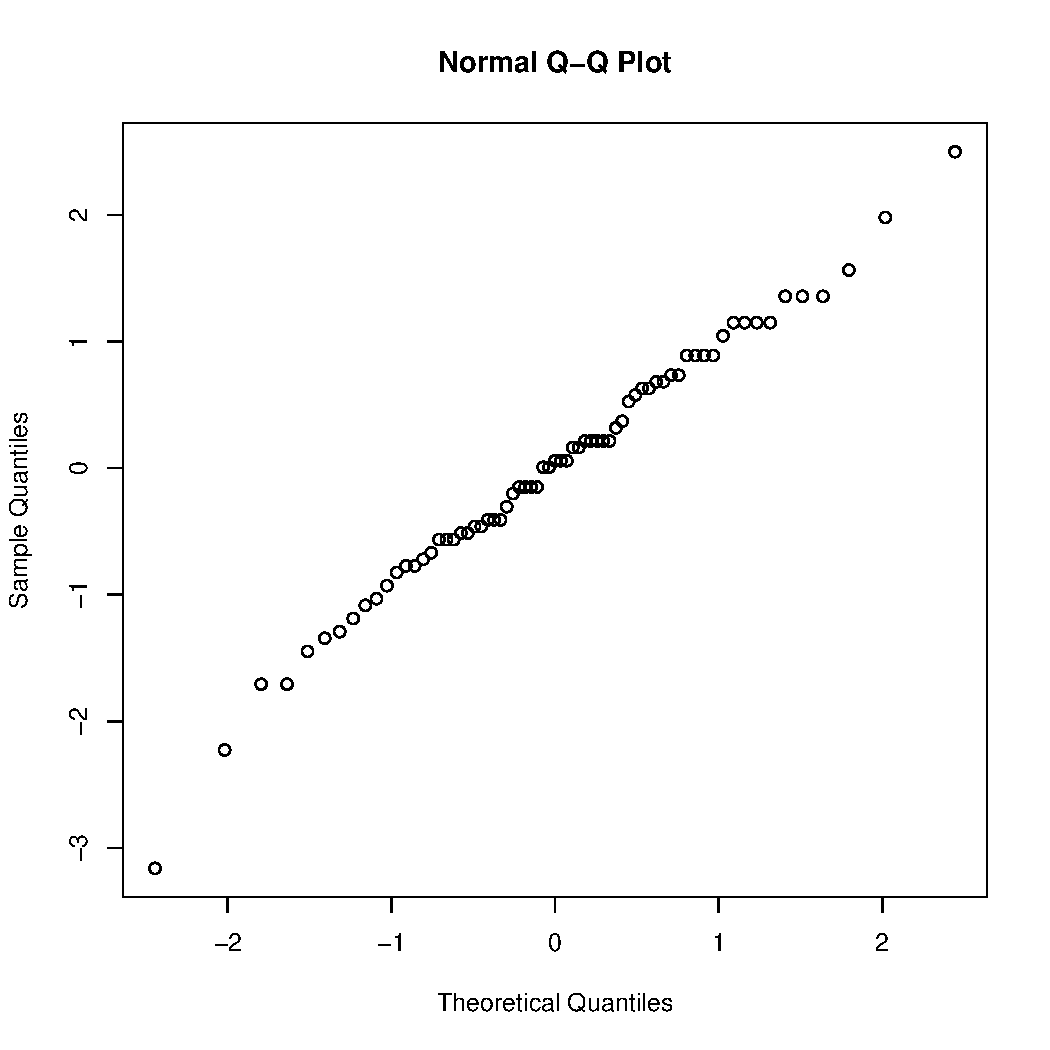
\includegraphics[width=0.95\columnwidth]{qqnorm}
\caption{Normal quantile-quantile plot for the standardized experimental data}
\end{figure}

\subsection{Selection of the best set of parameters}
We then proceed to choose the best set of parameters amongst the candidates.

We generate 10 samples for each set using the scripts \texttt{tenAveragedTestRBM.m} and \texttt{tenAveragedTestRBM\_noreg.m}. These scripts train 10 RBMs with hyperparameter set $S$ and tests them on our training set (\texttt{data\_val}). For each group, the 10 samples are drawn from the same normal distribution. We compare the means of the samples using two-samples T-Test to choose the set that has the lowest mean error.

\begin{table}
\resizebox{\columnwidth}{!} {
\begin{tabular}{|c|c|c|c|c|c|c|}
\hline
Sdisc & S0 & S1 & S2 & S3 & S4 & S5\\
\hline
32.067 & 32.995 & 32.023 & 32.111 & 32.641 & 31.979 & 31.935\\
33.304 & 32.641 & 32.023 & 32.288 & 32.067 & 31.979 & 31.184\\
32.862 & 34.231 & 31.670 & 32.155 & 32.067 & 31.493 & 32.332\\
33.436 & 33.525 & 31.890 & 32.332 & 32.155 & 31.493 & 32.332\\
32.730 & 32.641 & 31.935 & 31.714 & 32.774 & 32.023 & 31.316\\
33.436 & 32.509 & 30.786 & 31.493 & 31.670 & 32.730 & 31.625\\
32.553 & 32.862 & 32.288 & 32.332 & 33.436 & 31.802 & 31.360\\
32.818 & 32.332 & 31.802 & 31.537 & 32.244 & 32.420 & 31.670\\
32.597 & 33.171 & 32.155 & 32.023 & 32.332 & 31.095 & 31.228\\
33.348 & 32.951 & 31.051 & 31.670 & 32.067 & 32.200 & 32.067\\
\hline
\textbf{32.915} & \textbf{32.986} & \textbf{31.762} & \textbf{31.966} & \textbf{32.345} & \textbf{31.921} & \textbf{31.705}\\
\hline
\textit{0.4570}  &  \textit{0.5563}  &  \textit{0.4809}  &  \textit{0.3319} &   \textit{0.4941}  &  \textit{0.4785} &   \textit{0.4406}\\
\hline
\end{tabular}
}
\caption{Classification error on the test set on 10 runs for each parameter set. Average in bold. Standard deviation in italic.}
\end{table}

The results of the pair-wise tests are presented in the matrix below where:
\begin{itemize}
\item 0 indicates the test accepted the null hypothesis $H_0$: the samples have equal mean at the 5\% confidence level
\item 1 indicates we reject $H_0$ and accept $H_1$: the samples have different means
\end{itemize}
\[
\begin{matrix}
\mathcal{S}_{disc} & \mathcal{S}_0 & \mathcal{S}_1 & \mathcal{S}_2 & \mathcal{S}_3 & \mathcal{S}_4 & \mathcal{S}_5\\
0  &   0  &   1 &    1  &   0  &   1  &   1\\
0  &   0  &   1 &    1  &   1  &   1  &   1\\
1  &   1  &   0 &    0  &   1  &   0  &   0\\
1  &   1  &   0 &    0  &   1  &   0  &   0\\
0  &   1  &   1 &    1  &   0  &   0  &   1\\
1  &   1  &   0 &    0  &   0  &   0  &   0\\
1  &   1  &   0 &    0  &   1  &   0  &   0
\end{matrix}
\]

We also conducted Fisher F-Tests on the variances of the samples but no sample had a variance significantly different than the others at the 5\% confidence level. There are probably not enough samples, or this might not be a relevant quantity to measure.

\section{Conclusion}

Based on the above results, we can only conclude that $\mathcal{S}_1$, $\mathcal{S}_2$, $\mathcal{S}_4$, and $\mathcal{S}_5$ have similar performance and perform better than the other parameter sets.

We can also see that $\mathcal{S}_{disc}$, $\mathcal{S}_0$, and $\mathcal{S}_3$ also have similar performance. This might indicate that using regularization techniques such as introducing a weight decay coefficient doesn't automatically improve the classification error on the test set.

\vspace{1em}

It is difficult to draw any conclusion by comparing the results on the testing set with the performance on the validation set shown in table 1 since the optimization procedure didn't involve averaging the performance of several runs for a given set of parameters.

We can however notice that the performance of $\mathcal{S}_1$ on the validation set shown in table 1 is very close to its average performance on the training set as shown in table 2. On the contrary, $\mathcal{S}_5$ has the best average performance in table 2 but performs quite poorly in table 1. Similar behaviour is observed for $\mathcal{S}_2$ and $\mathcal{S}_4$. This might be a sign that these sets would perform worse than $\mathcal{S}_1$ on average but the data we have doesn't back this assertion and we cannot rely on a single sample to conclude.

One interesting way of better discriminating the four sets would be to gather more data, and to perform better comparisons of the variances since a low variance could translate in a more consistent classification error.

\section{A note on the code}

\begin{itemize}
\item File \texttt{TrainAndTest.m} trains an RBM with the parameters from $\mathcal{S}_5$ and output the prediction error on the test set (\texttt{data\_val}).

\item Files \texttt{tenAveragedTestRBM.m} and its noreg counterpart train and test ton RBMs for a given parameter set.

\item SMAC must be run as follows: \texttt{./smac --scenario-file FILE}. An optional parameter \texttt{--seed} allows to distinguish more easily between runs (used for naming the folders in \texttt{smac-output}).

\item The file \texttt{rbm.mat} contains a pre-trained RBM using the parameters from $\mathcal{S}_5$.
\end{itemize}

A few \texttt{csv} files are provided as evidence of the different experimentations.

\subsection{Troubleshooting}

SMAC will fail to launch if the path to its script contains spaces.

The MATLAB functions called by the wrappers SMAC uses require Medal to be in the same folder as them.

\end{document}
